\documentclass{article}
\usepackage{parskip}
\usepackage{indentfirst}
\setlength{\parindent}{1cm}
\renewcommand{\baselinestretch}{1.4}

\usepackage{graphicx}
\usepackage{caption}
\usepackage{subcaption}
\usepackage{url}
\usepackage{enumitem}
\usepackage{adjustbox}
\usepackage{amssymb}

\usepackage{hyperref}
\hypersetup{
    colorlinks=true,
    linkcolor=red,
    filecolor=blue,      
    urlcolor=blue,
    citecolor=red
}
 
\usepackage[
    top    = 3cm,
    bottom = 2cm,
    left   = 2.8cm,
    right  = 2.8cm]{geometry}
\usepackage[utf8]{inputenc}

\usepackage{fancyhdr}
\pagestyle{fancy}
\renewcommand{\headrulewidth}{0pt}
\fancyhf{}
\lhead{PHYS3051}
\rhead{Desiree Vogt-Lee}
\cfoot{\thepage}

\title{Implementing the Klein Gordon Equation on a Quantum Computer}
\author{Desiree Vogt-Lee, 44354471}
\date{10 June, 2019}

\begin{document}
	\maketitle
	\begin{center}
	    All components of this project including code, Jupyter Notebooks, LaTeX files and images can be found in my \href{https://github.com/desireevl/PHYS3051}{Github repository}, please check this out for reference.
	\end{center}


\section{The Klein Gordon Equation}
The Klein Gordon equation set out to unify quantum mechanics and special relativity and ultimately led to the creation of the Dirac equation from which quantum field theory was born.

The Klein Gordon (KG) equation is unable to describe a particle as the Schrodinger equation does due to there being no conserved probability. 

\begin{equation}
\frac{1}{c^2}\frac{\partial^2}{\partial t^2}\psi - \nabla^2 \psi + \frac{m^2c^2}{\hbar^2}\psi = 0
\end{equation}

The Schrodinger equation is a first order equation in the time derivative where its' wavefunction is able to predict its future evolution. The Klein Gordon equation on the other hand is second order in the time derivative and the boundary condition for the field must be given to work out the field evolution. The KG equation also allows energy to be a negative value which can't be eliminated by limiting to only positive initial conditions due to run off effects that result in particles with E $< 0$. The Dirac equation was Dirac's attempt to create an equation that had a first order time derivative and was relativistic \cite{uqnotes}.



The Klein paradox arises from using the Dirac equation to solve the problem of electron scattering from a barrier potential. Under non-relativistic circumstances, the electron would tunnel into the barrier. However if the barrier potential is greater than $mc^2$, the particle is able to penetrate the barrier as if it were transparent \cite{klein}.



This report will be based off a paper titled \textit{Quantum Simulation of Klein Gordon Equation and Ob-servation of Klein Paradox in IBM Quantum Computer} by Manik, K et al. (2018) \cite{manik} which aimed to simulate the time dependent Klein Gordon equation in a barrier potential on a quantum computer to see the tunneling of both the particle and anti-particle with the Klein Paradox.

The present report aims to replicate results, justify decisions made in the original publication and offer criticism and suggestions. 

\subsection{Klein Gordon Equation in Unitary Form}
To implement the KG equation on a quantum computer, it must be written in terms of unitary operators \cite{manik}. To do this we start with the equation for a Hamiltonian in terms of mass of a particle (m), momentum operator ($\hat{p}$), potential (V), speed of light (c), identity matrix (I) and Pauli matrices ($\sigma_{1,2,3}$):

\begin{equation}
\hat{H}=\frac{\sigma_{3}+i \sigma_{2}}{2 m} \hat{p}^{2}+\sigma_{3} m c^{2}+I \hat{V}
\end{equation}

\noindent By using the vector: 
\[\varphi=\left[\begin{array}{l}{\phi} \\ {\chi}\end{array}\right]\]

\noindent We can solve two simulataneous equations, resulting in:
\[\hat{H}_{1} \phi=\frac{\hat{p}^2}{2m}(\phi+\chi)+(mc^2+\hat{V}) \phi\]
\[\hat{H}_{2} \chi=-\frac{\hat{p}^2}{2m}(\phi+\chi)+(-mc^2+\hat{V}) \chi\]

\noindent These equations then need to be represented as a time evolution equation which can be done by taking the second order Trotter-Suzuki (TS) decomposition \cite{trotter} of the Hamiltonian:
\[|\psi(x, t+\delta)\rangle= e^{-i \hat{H}_{i} t}|\psi(x, t)\rangle\]

The TS decomposition equation simplifies calcuations of matrix exponentials that are required to solve the time dependent Schrodinger equation by proposing a way to rewrite exponentials to unitary operators allowing for less intensive computation:

\[e^{-i \hat{H}_{1} t}=e^{-i\left(\frac{\tilde{p}^{2}}{2 m}(\square+\square)+\hat{V}_{1}\right) t}\]
\[e^{-i \hat{H}_{2} t}=e^{i\left(\frac{\tilde{p}^{2}}{2 m}(\square+\square)-\hat{V}_{2}\right) t}\]

Where $\square$ is the component of the wavefunction. Each momentum operator can be expressed using the quantum Fourier transform and its inverse in momentum space, which is explained in the IBM Research Report (1994) \cite{ibm} to result in the final unitary operators that can be implemented on the quantum computer:
\begin{equation}
e^{-i \hat{H}_{1} t}=F^{-1} e^{-i \hat{p}_{p}^{2} \square} . F . F^{-1} \cdot e^{-i \hat{p}_{p}^{2} \square} F \cdot e^{-i V_{1} \sigma_{z} t}
\end{equation}

\begin{equation}
e^{-i \hat{H}_{2} t}=F^{-1} e^{i \hat{p}_{p}^{2} \square} . F . F^{-1} \cdot e^{i \hat{p}_{p}^{2} \square} F \cdot e^{-i V_{2} \sigma_{z} t}
\end{equation}

\section{Quantum Computing}
Quantum computing is the melding together of quantum mechanics and classical computation. The computer chips used in quantum computers use the same fundamental components as that of their classical counterparts, however are pieced together in a way which allow quantum-bits, or qubits, to be used instead of bits. 

A fundamental flaw in the current design of quantum computers is the large amount of error that is created due to noise and decoherence, which increases with the number of qubits used. This severely limits the computation that can be performed with a negligable amount of error, as at some point, the current error correcting codes will have little effect. 

Many believe that quantum computation is the future. Due to the superposition and entanglement properties these qubits can possess, all sorts of optimisation and new algorithms can be created, which would have significant impact on many fields of technology. For example, modern cryptography is centered around the assumption that creating incredibly long numbers take current computers an impossibly long time to factorise. Using Shor's algorithm, a quantum computer would be able to factorise a number in polynomial time, exponentially faster than the best classical algorithm, and thus being able to break modern cryptography. \cite{minutephysics}

At present, this is all merely a premonition; as although there exists many quantum algorithms, the error is too great and the number of qubits too little to be able to use them. I believe that applying the Klein Gordon equation on a quantum computer is useful in showing the present capabilities of this new technology as well as just being a really interesting application.

\subsection{Gates}
To modify the state that a qubit is in, a gate or procession of gates can be applied to it. The quantum gates are similar to the logic gates present in classical computing, but work with the quantum nature of the qubit. To easily conceptualise the effect of a quantum gate, a geometric representation called the Bloch sphere is used, where the poles of the sphere represent the standard basis vectors $|0\rangle$ and $|1\rangle$.

\begin{figure}[!htb]
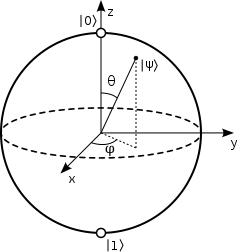
\includegraphics[scale=0.55]{../images/bloch_sphere}
  \centering
  \caption{Bloch Sphere \cite{blochsphere}}
\end{figure}

In classical computation, the NOT gate simply flips a given bit state: a 1 will be transformed to a 0 and vice versa. In quantum computing there is an equivalent X gate which when applied to a qubit in the $|0\rangle$ state, performs a rotation about the x axis on a Bloch sphere by $\pi$ radians resulting in the $|1\rangle$ state when measured (for more detailed explanation on the fundamental gates and terminology, please see my \href{https://desireevl.github.io/archive/2019/04/03/quantum-intro.html}{blog post}).

Here I will briefly explain the gates that will be used to create the circuit that implements the Klein Gordon equation (minus those explained in my blog post):
\newline

\begin{itemize}[labelindent=1.5em,labelsep=0.9cm,leftmargin=*]
	\item\adjustbox{valign=t}{
\includegraphics[width=0.7cm]{../images/t_gate}} {} {} {} {}  T: performs a $\frac{\pi}{4}$ rotation about the z axis, which is equivalent to a quarter of one Z gate operation. This gate acts on the phase of the qubit and is represented by the matrix: 
\[T=\left(\begin{array}{ll}{1} & {0} \\ {0} & {e^\frac{i\pi}{4}}\end{array}\right)\]
	\item\adjustbox{valign=t}{
\includegraphics[width=0.7cm]{../images/tdagger_gate}} {} {} {} {}  $T^\dagger$: simply the opposite of the T gate and applies a $-\frac{\pi}{4}$ rotation about the z axis \cite{qiskitt}.
	\item\adjustbox{valign=t}{
\includegraphics[width=0.7cm]{../images/u1_gate}} {} {} {} {}  $U_1$: performs a unitary rotation on the state vector where the continuous phase can be specified. It is represented by the following matrix and as can be seen, is of a similar to that of the T gate, suggesting that a $U_1(\frac{\pi}{4})$ gate is equivalent to a T gate.
	\[U_1(\lambda) = \left(\begin{array}{ll}{1} & {0} \\ {0} & {e^{i \lambda}}\end{array}\right)\]
	\item\adjustbox{valign=t}{
\includegraphics[width=0.7cm]{../images/u3_gate}}  {} {} {} {} $U_3$: used to perform arbitrary unitary operation, where the $\theta$, $\psi$ and $\lambda$ position of the vector on the Bloch sphere can be modified to any value. This is the most general form of a single qubit unitary operation and is represented in matrix form as \cite{qiskitu}:
	\[U=\left(\begin{array}{cc}{\cos (\theta / 2)} & {-e^{i \lambda} \sin (\theta / 2)} \\ {e^{i \phi} \sin (\theta / 2)} & {e^{i \lambda+i \phi} \cos (\theta / 2)}\end{array}\right)\]
	\item R
	\[R = \left(\begin{array}{cc}{1} & {0} \\ {0} & {e^{2 \pi i / 2^{k}}}\end{array}\right)\]
	\item\adjustbox{valign=t}{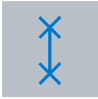
\includegraphics[width=0.7cm]{../images/swap}} {} {} {} {}  SWAP: operates on a pair of qubits and swaps their state.
    \item\adjustbox{valign=t}{
\includegraphics[width=0.7cm]{../images/measurement_gate}} {} {} {} {} Measurement: used at the end of the circuit to measure the outcome of the states in the z basis.
    \item\adjustbox{valign=t}{
\includegraphics[width=0.7cm]{../images/barrier}} {} {} {} {} Barrier: directives which inform the complier not to optimise across barriers. They serve the purpose of keeping gates, especially measurement gates, in their place and are as well used as a visualisation tool to separate parts of the circuit.
\end{itemize}


\section{The Circuits}
Equations xxxxxx and xxxxxxx can be broken up and implemented into a circuit. As we are attempting to recreate results from Manik, K. (2018) \cite{manik}, we will take $V_1 = 12$ and $V_2 = 10$. No justification is given as to why these potentials are used. The circuits described in Figures xxxxx and xxxxxxxxx have their components separated by barriers and we will refer to each section in the order they appear starting at section 1 where the U1 gate appears. 

The first and last U1 gates (section 1 and 8) implement the potential term in the Klein Gordon equation. Then as per Equations xxxxx and xxxxxxxxx, inverse QFTs appear at sections 2 and 5 of the circuit and regular QTFs appear at sections 4 and 7 (explanation of these circuit implementations of the QFT can be seen shortly).

In the code there is an option to choose to run the circuit on a real IBM quantum computer or the simulator.

\begin{figure}[!htb]
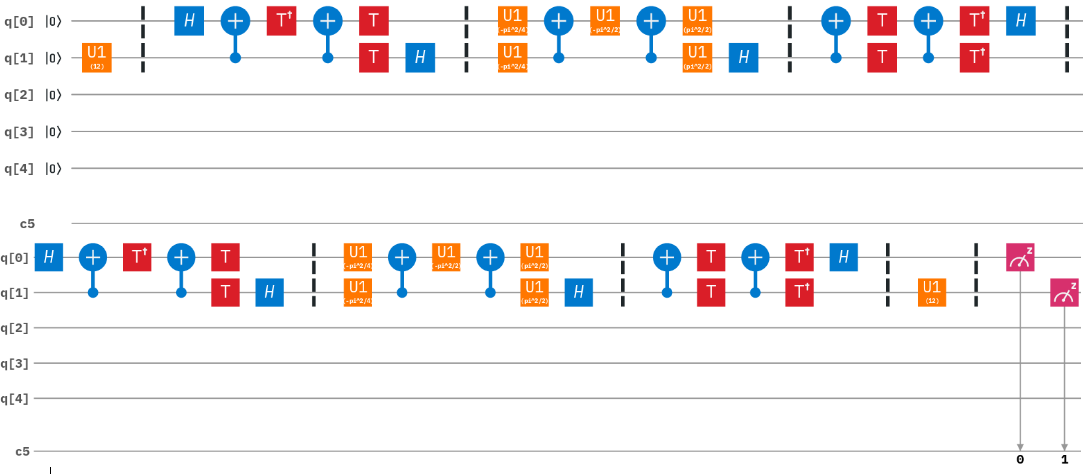
\includegraphics[scale=0.42]{../images/circuit1_colour}
  \centering
  \caption{Circuit 1 }
\end{figure}

\begin{figure}[!htb]
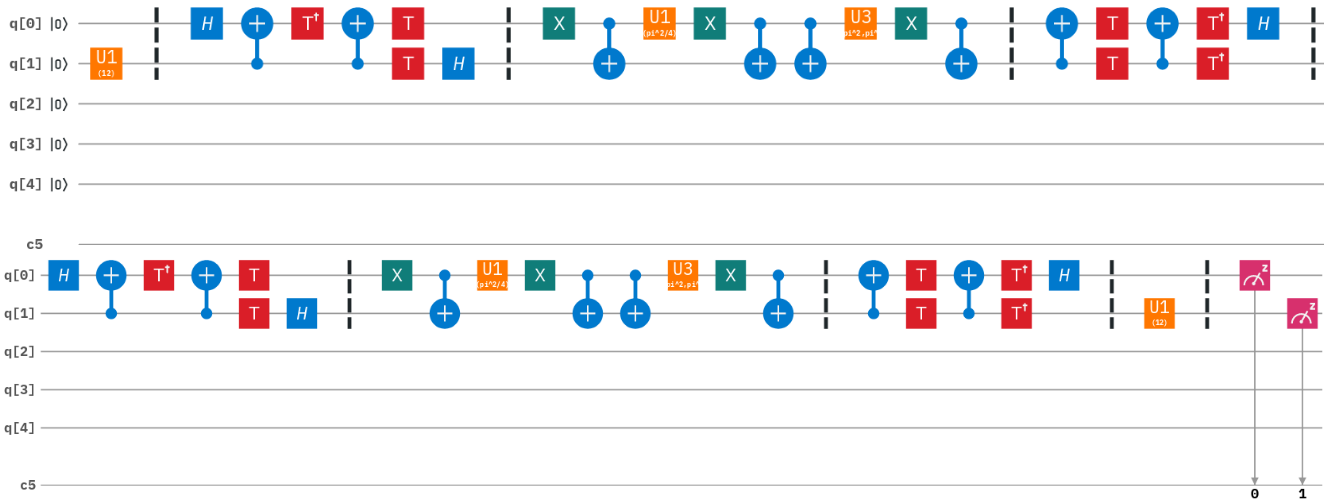
\includegraphics[scale=0.34]{../images/circuit2_colour}
  \centering
  \caption{Circuit 2}
\end{figure}

\subsection{Fast Fourier Transform}
The Fourier transform is able to decompose a function into its constituent functions, which has many practical applications including signal processing, analysis of differential equations and spectroscopy \cite{fourier}. One particular variation of Fourier transform of interest is the discrete Fourier transform (DFT) as it is computed using the fast Fourier transform (FFT) algorithm. The DFT computes a finite sequence of points of a function to its various frequency components, which although useful, is computationally expensive. The Cooley-Tucky \cite{turkey} FFT algorithm accelerates this process by splitting up the DFT problem into smaller parts and recognising a symmetry that exists between each even term and each odd term:

\begin{equation}
y_{k}=\sum_{n=0}^{N-1} x_{n} \cdot e^{-i 2 \pi k n / N}
\end{equation}

\[=\sum_{m=0}^{N / 2-1} x_{2 m} \cdot e^{-i 2 \pi k(2 m) / N}+\sum_{m=0}^{N / 2-1} x_{2 m+1} \cdot e^{-i 2 \pi k(2 m+1) / N}\]
\[=\sum_{m=0}^{N / 2-1} x_{2 m} \cdot e^{-i 2 \pi k m /(N / 2)}+e^{-i 2 \pi k / N} \sum_{m=0}^{N / 2-1} x_{2 m+1} \cdot e^{-i 2 \pi k m /(N / 2)}\]

\noindent Therefore instead of having to recompute the entirety of each term, only half of the subproblem needs to be computed. This method of dividing and computing half can be applied recursively until the vectors are small enough that the method no longer yields better results, at which point the computational complexity is $O(n\log{}n)$ (compared to the $O(n^2)$ of regular DFT) \cite{jvdp}.

\subsection{Quantum Fourier Transform}
The quantum Fourier transform is very similar to the FFT mentioned above. The quantum version acts on amplitudes of a quantum state and maps them to new amplitudes. The mathematical representation of the QFT is:

\begin{equation}
\alpha_{j}|j\rangle \rightarrow \alpha_{j}\left(\frac{1}{\sqrt{N}} \sum_{k=0}^{N-1} e^{2 \pi i \frac{k j}{N}}|k\rangle\right)
\end{equation}

As in with standard DFT, a delta function will be transformed to a sine function using a QFT. For a two qubit system, with one qubit in the $|1\rangle$ state and the other in the $|0\rangle$ state, $|10\rangle$ will transform into the following superposition: 

\begin{figure}[!htb]
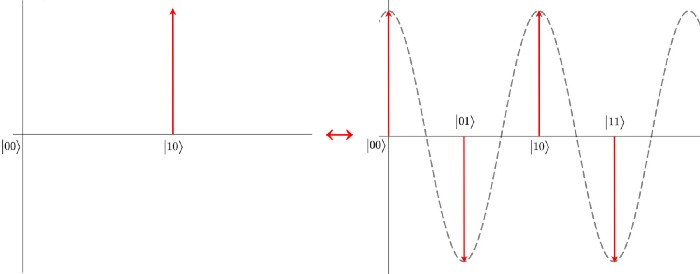
\includegraphics[scale=0.4]{../images/fourier}
  \centering
  \caption{Delta function transformed to a sine function of two qubits: $|10\rangle \rightarrow |00\rangle-|01\rangle+|10\rangle-|11\rangle$ \cite{jonathan}}
\end{figure}

Just as the FFT is performed iteratively on subproblems, so is the QFT: Equation xxxxxxxxxxxxxxx can be broken down into the following expression which allows for easier understanding of how the equation can be implemented as gates on a quantum circuit.

\begin{equation}
\left|j_{1} \cdots j_{n}\right\rangle \rightarrow \frac{\left(|0\rangle+ e^{2 \pi i 0 . j_{n}}|1\rangle\right)\left(|0\rangle+ e^{2 \pi i 0 . j_{n-1} j_{n}}|1\rangle\right) \cdots\left(|0\rangle+ e^{2 \pi i 0 . j_{1} j_{2} \cdots j_{n}}|1\rangle\right)}{2^{n / 2}}
\end{equation}

The first Hadamard in the following circuit representation of Equation xxxxxxxxxx puts the system into the superposition state required (the $1/\sqrt{2}$) and the following multiplications are implemented using the R controlled phase gates. The pattern apparent in the circuit indicates the recursive nature of the algorithm. The swap gate can be applied either at the beginning or end of the system as it is just required that the states of the two qubits are swapped prior to measurement and its position has no effect on the outcome.

\begin{figure}[!htb]
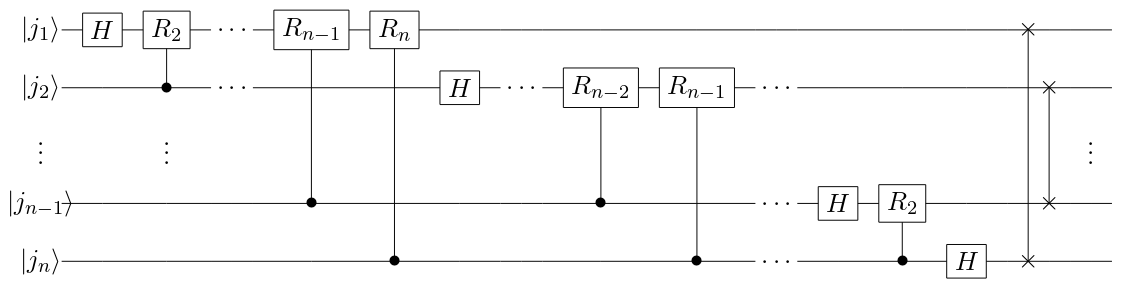
\includegraphics[scale=0.35]{../images/qft_circuit}
  \centering
  \caption{QFT circuit implemented on an n qubit system \cite{jurgen}.}
\end{figure}

As our implementation of the Klein Gordon equation only uses two qubits, the quantum Fourier transform on two qubits is represented by the following circuit.


Like the classical Fourier transform, the quantum Fourier transform is reversible as well as unitary.

\section{Exploration}
The time step interval (t) in Equation xxxxxx and xxxxxxxx was not provided in the original paper. I reached out to the author who was unable to provide the original values for these time steps however noted that the time started at t=0 and increased at a very small rate linearly. After trial and error of various time steps, the time step that yielded the most similar heatmap was t=0.02. Despite the long time spent trying to work out the time step, the resulting heatmaps were significantly different to those gained in the reference paper (see Figure xxxxxxxx).

\begin{figure}[!htb]
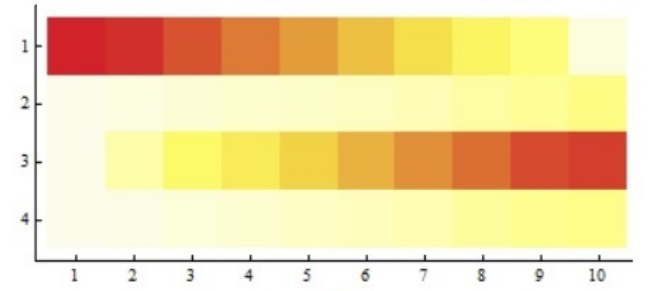
\includegraphics[scale=0.35]{../images/org_circ1}
  \centering
  \caption{Circuit 1 heatmap results from original paper \cite{manik}.}
\end{figure}

As the timestep used by the author was most likely chosen to best show the evolution of the states over time, it is not significantly important to get it exactly correct. However even with smaller timesteps/greater evolution time (these can be easily modified in the code \cite{ipynb}), the pattern found in the original heatmap was unable to be replicated which might suggest an error in the implementation of the KG equation.

The original paper used the IBM Q simulator exclusively, speculatively due to the ideal, consistent results and fast output as opposed to the real device. In the code I have written for these circuits \cite{ipynb}, there is a toggle to run the circuit on either the IBM Q simulator or the IBMQx2 two qubit quantum computer. Below are the results of running the exact circuit from the reference paper on both devices. 

\begin{figure}
\centering
\begin{subfigure}{.5\textwidth}
  \centering
  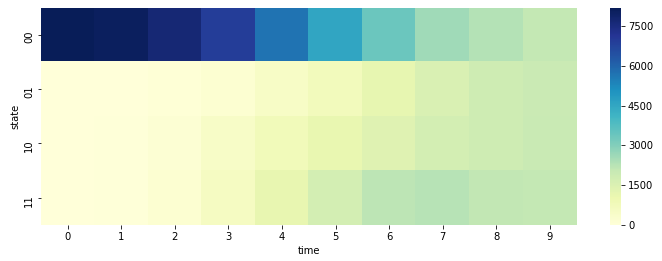
\includegraphics[width=0.9\linewidth]{../images/circ1_heatmap_sim}
  \caption{Circuit 1 run in the simulated IBMQ environment}
  \label{fig:sub1}
\end{subfigure}%
\begin{subfigure}{.5\textwidth}
  \centering
  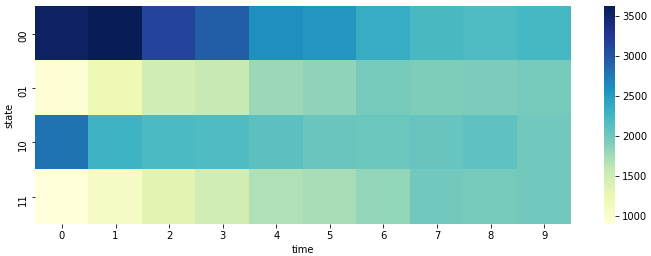
\includegraphics[width=0.9\linewidth]{../images/circ1_heatmap_real}
  \caption{Circuit 1 run on the real IBMQx2 device}
  \label{fig:sub2}
\end{subfigure}
\caption{Circuit 1 run on different devices.}
\label{fig:test}
\end{figure}

As seen from Figure xxxxxxxxxxx, there is significant difference between the results from the simulated and real devices. Although some difference is to be expected due to an increase of error and uncertainty in real qubits, such a large discrepancy was unforseen. 

The QFT and IQFT implementations in the circuit by Manik, K (2018) \cite{manik} is different that mentioned in Section  

\section{Results}
The expected results of the implementation of the Klein Gordon equation is that for a pair of qubits at t=0, both qubits start in a $|00\rangle$ state and cross the barrier potential as expected by the Klein paradox. In the reference paper results this phenomenon is clearly observed as the particle and anti-particle tunnel at the high and low potentials, leading to the final state of the particle being $|10\rangle$. The author of the reference paper claims that the Klein paradox and tunneling effects are due to the chosen strong potential values and setting $mc^2=1$. 

In this report, I was unable to reproduce the exact results gathered in the Manik, K. (2018) \cite{manik} paper. Using the IBMQ simulator, the qubit state started at $|00\rangle$ and ended spread out across the range of possible states however with slightly stronger appearance in the $|11\rangle$ state. 

maybe you can't get tunneling with ideal simulator

\bibliography{refs.bib}
\bibliographystyle{ieeetr}



\end{document}
